\chapter{Link Discovery}

Das folgende Kapitel beschäftigt sich mit den im Rahmen dieser Arbeit unternommenen Schritten zur Link Discovery, also dem Finden von Beziehungen zwischen Wörtern und Wortgruppen. Dazu zählen die Generierung eines Ausgangsgraphen aus Tag-Daten sowie dessen Anreicherung durch die Integration weiterer interner und externer Datenquellen.

\section{Tags}

Den Ausgangspunkt für den in \ref{solution} beschriebenen Lösungsansatz stellen die Daten des Tag-Systems dar. Diese werden in \ref{tag-system} ausführlich beschrieben. Aus diesen Daten wird im ersten Schritt der Graph erstellt, in diesen in allen weiteren Schritten weitere Daten integriert werden. Die in diesem Graph enthaltenen Knoten stellen also die Kriterien für die Abfrage der weiteren Datenquellen dar.

Um den Ausgangsgraphen zu berechnen, sind die Schritte des Imports, der Bereinigung, der Reduktion, der Transformation und der Integration notwendig \cite{hkp2012}, welche im folgenden genauer beschrieben werden.

\subsection{Import}

Die Daten liegen im Quellsystem in relationaler Form vor. Somit existieren Tabellen für die Tags, Dokumente und Verknüpfungen zwischen ebenjenen. Da der Inhalt der Dokumente nicht relevant für die Link Discovery mittels Kookkurrenz sind, genügt es, die Tabellen der Tags und Verknüpfungen zu importieren.

Die Tags liegen in der Form \((i, s, l)\) vor, wobei \(i\) den eindeutigen Bezeichner des Tags, \(s\) die Zeichenkette und \(l\) die Sprache des Tags repräsentieren.

Die Verknüpfungen sind durch Tupel der Form \((i, t, d_t, d_i)\) repräsentiert, wobei \(i\) der eindeutige Bezeichner der Verknüpfung selbst ist. \(t\) ist der Bezeichner des Tags, \(d_t\) der Typ des Dokuments und \(d_i\) der Bezeichner des Dokumentes. \(d_t\) und \(d_i\) bilden also den zusammengesetzten Schlüssel des getaggten Dokumentes. 
 
\begin{figure}
\centering
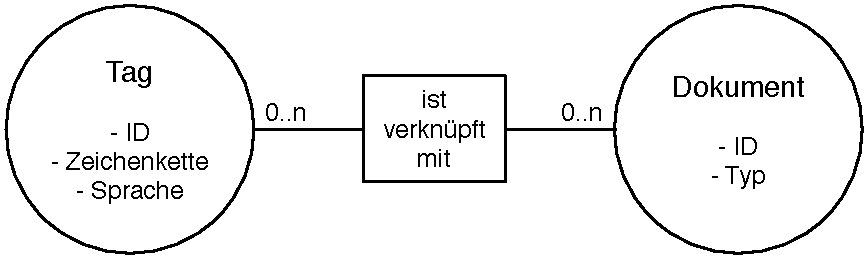
\includegraphics[width=0.6\textwidth]{tag_source_erd}
\caption{Tag-Quelldaten als Entity-Relationship Diagramm}
\label{fig:tag_source_erd}
\end{figure}

Die importierten Quelldaten sind in Abbildung \ref{fig:tag_source_erd} als Entity - Relationship Diagramm abgebildet. Nach dem Import stehen \num{2072079} Tags und \num{71938905} Verknüpfungen zur Verfügung.

\subsection{Bereinigung}

An den Tag-Daten liegen die in \ref{quality} genannten Defekte in Hinblick auf die Datenqualität vor. Diese sollten in einem Bereinigungsschritt reduziert werden. Hierbei liegt das Hauptaugenmerk auf der Erkennung von Duplikaten und später nicht verwertbaren Zeichenketten. Alle durchgeführten Maßnahmen zur Bereinigung beziehen sich hierbei auf die Eigenschaft \(s\) des Tags, also der Zeichenkette selbst.

In den unbereinigten importierten Daten existieren keine Duplikate in der Art, dass eine Paarung aus Zeichenkette und Sprache immer nur genau einmal in den Daten vorhanden ist. Jedoch enthalten viele der Tags nicht weiter verwertbare Zeichen wie nicht druckbare ASCII Zeichen, Anführungszeichen, Satzzeichen, Sonderzeichen sowie überflüssige Leerzeichen am Anfang und Ende der Zeichenkette. Außerdem existiert in den importierten Daten eine Unterscheidung zwischen Groß- und Kleinschreibung. Diese Unterscheidung bringt im Kontext der Link Discovery keine Vorteile und kann somit entfernt werden.

\begin{table}
\centering
\begin{tabular}{|l|l|}
    \hline
    Rohdaten & Bereinigte Daten \\
    \hline
    \textbackslash u0003\textbackslash r\textbackslash nregenbogen & regenbogen \\
    RegenBogen & regenbogen \\
    "Regenbogen" & regenbogen \\
    regenbogen +einhorn & regenbogen einhorn\\
    \hspace{10 mm} regenbogen & regenbogen \\
    regenbogen & regenbogen \\
    \hline
\end{tabular}
\caption{Beispiele für die Tag-Bereinigung}
\label{tab:tag_cleaning}
\end{table}

Somit besteht der Bereinigungsschritt darin, nicht verwertbare Zeichen zu entfernen und alle Großbuchstaben in Kleinbuchstaben umzuwandeln. Dadurch entstehen Duplikate, welche im darauf folgenden Reduktionsschritt entfernt werden können. In Tabelle \ref{tab:tag_cleaning} sind einige Beispiele für die Bereinigungen aufgeführt. Dabei ist gut zu erkennen, dass durch die Bereinigungen Duplikate erzeugt werden.

\subsection{Reduktion}

Der Reduktionsschritt dient zur Einschränkung der Gesamtdaten auf eine nützliche oder handhabbare Menge. Außerdem kann durch Reduktion auch die Datenqualität verbessert werden.

Im Fall der Tag-Daten liegt das Hauptaugenmerk im Reduktionsschritt auf der Entfernung von Duplikaten, die bei der Bereinigung entstanden sind. Dabei muss gleichzeitig sicher gestellt werden, dass keine Informationen über die Verwendung der Tags verloren gehen. Somit besteht die Duplikatentfernung der Tags im Zusammenführen von Datensätzen mit gleichen Zeichenketten und Sprachen. Dabei werden auch die Verwendungen der Tags zusammengeführt.

Werden die Verknüpfungen zweier Tags mit Dokumenten zusammengeführt, können auch dabei wieder Duplikate entstehen. Diese müssen in diesem Fall entfernt werden, da ein Tag nicht mehrmals mit einem Dokument verknüpft werden kann. Das Zusammenfühen von Tags ist exemplarisch in Abbildung \ref{fig:tag_reduction} dargestellt.

\begin{figure}
\centering
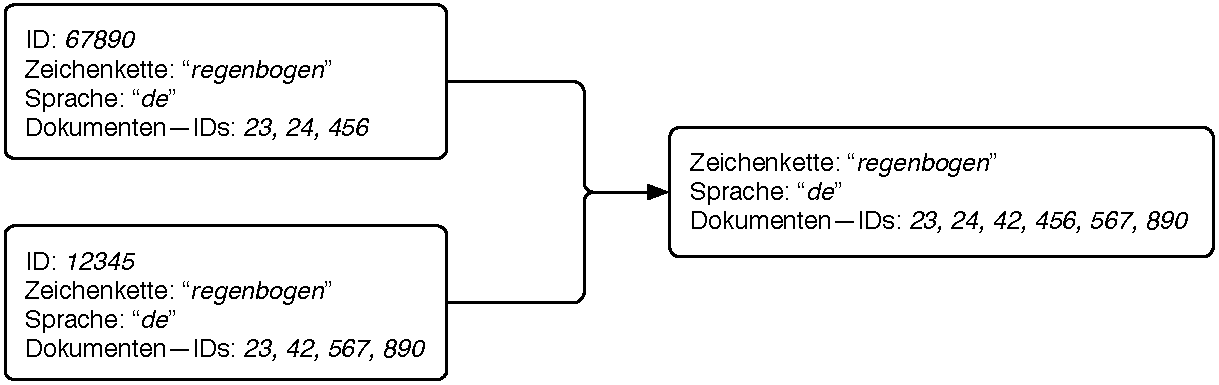
\includegraphics[width=0.7\textwidth]{tag_reduction}
\caption{Beispiel für das Zusammenführen der bereinigten Tags}
\label{fig:tag_reduction}
\end{figure}

Eine weitere im Rahmen dieser Arbeit unternommene Maßnahme zur Datenreduktion bestand darin, sich auf die Menge der Tags zu beschränken, deren Attribut \(l\) den Wert \emph{de} besitzt. Praktisch handelt es sich dabei um alle Tags, die als deutsch gekennzeichnet in der Datenbank gespeichert sind. Diese Einschränkung wurde vorgenommen, um die zu verarbeitende Datenmenge überschaubar zu halten.

Ein letzter Reduktionsschritt besteht in der Entfernung der Tags, deren Zeichenketten eine Länge von \num{1} besitzen, da in der deutschen Sprache keine einbuchstabigen Wörter existieren.

Nach der beschriebenen Reduktion befinden sich noch \num{314351} Tags und \num{23255714} Verknüpfungen in der Datenbank. Dies entspricht einer Reduktion von ca. \num{68} Prozent gegenüber der importierten Menge von Objekten.

\subsection{Transformation}

Der Transformationsschritt beschreibt die Überführung der Daten in die Form, die für das Ergebnis benötigt wird. Im Falle der Tag-Daten bedeutet dies eine Umformung in die Form des Kokkurrenzgraphen, also die Erzeugung von Knoten- und Kantenobjekten. Die Umsetzung dieser Transformation mittels des Programmiermodells MapReduce wurde in \ref{mapreduce_cooccurence} genauer beschrieben.

Um die vorhandenen Informationen später einfach nutzbar zu machen, erscheint es sinnvoll, die Knoten mit allen verfügbaren Daten anzureichern. Dazu gehören bei den Tags die Sprache und Zeichenkette, sowie Informationen darüber an welche Dokumente der Tag verwendet wurde. Diese Informationen lassen sich in einer dokumentenbasierten Datenbank leicht abbilden.

Je Tag wird ein Datenbankdokument erzeugt, dass den Knoten repräsentiert. Dieses besitzt als Attribute zum einen die Zeichenkette und die Sprache des Tags, aus dem es erzeugt wurde. Zum anderen wird ein Unterdokument hinzugefügt, welches weitere Eigenschaften des Ausgangstags beschreibt. Die umfasst die Anzahl der Verwendungen und die eindeutigen Bezeichner der Dokumente, die mit dem Tag getaggt wurden. Außerdem kann im Transformationsschritt für jeden Knoten ein global eindeutiger Bezeichner erzeugt werden, um das spätere Referenzieren der Knoten einfacher zu machen. Zeichenkette und Sprache des Knotens stellen einen zusammengesetzten Schlüssel dar und sind in der Knotenmenge eindeutig. Der Aufbau der Knoten ist schemahaft in Abbildung \ref{fig:tag_transform_node} dargestellt. Listing \ref{lst:tag_transform_node} zeigt ein Beispiel für ein in der Datenbank abgelegtes Knotendokument.

\begin{figure}
\begin{center}
    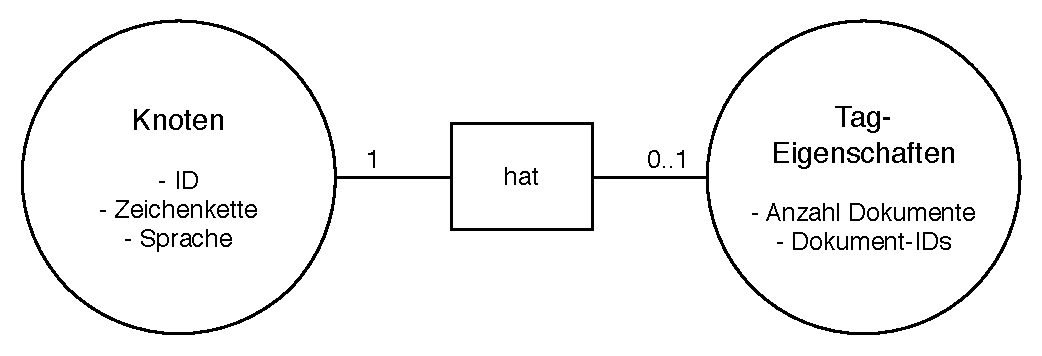
\includegraphics[width=0.7\textwidth]{tag_transform_node}
\end{center}
\caption{Aufbau der aus den Tag-Daten erzeugten Knoten}
\label{fig:tag_transform_node}
\end{figure}

\begin{lstlisting}[language=json, label={lst:tag_transform_node}, caption={Tag-Knoten als JSON-Dokument}]
{
    "_id" : ObjectId("51efc20147cae77dfc02e0ac"),
    "language" : "de",
    "string" : "mama",
    "tagProperties" : {
        "occurenceCount" : 3,
        "articleCount" : 2,
        "designCount" : 1,
        "articleIDs" : [
            24231101,
            24231105
        ],
        "designIDs" : [
            15514592
        ]
    }
}
\end{lstlisting}

Die Erzeugung der Kanten erfolgt dann wie in Abschnitt \ref{mapreduce_cooccurence} beschrieben. Dabei werden für jedes gemeinsame Auftreten von zwei Tags zwei Datenbankdokumente erzeugt. Dieses beschreiben gerichtete Kanten zwischen den Tags, die ein gemeinsames Auftreten der Tags repräsentieren. Neben Quell- und Zielknoten enthält eine Kante den Kantentyp sowie weitere Informationen über die Art der Verbindung. Im Fall von Kookkurrenzkanten ist dies zum einen die absolute Anzahl gemeinsamer Vorkommen der Tags, zum anderen die in \ref{measures} beschriebenen Kookkurrenzmaße. Der Kantentyp ist aus der Berechnung folgend der Typ der Tag-Kookkurrenz. Der Aufbau der erzeugten Kanten ist in Abbildung \ref{fig:tag_transform_edge} dargestellt. Ein Beispiel JSON-Dokument für eine Kante ist in Listing \ref{lst:tag_transform_edge} zu sehen.

\begin{figure}
\centering
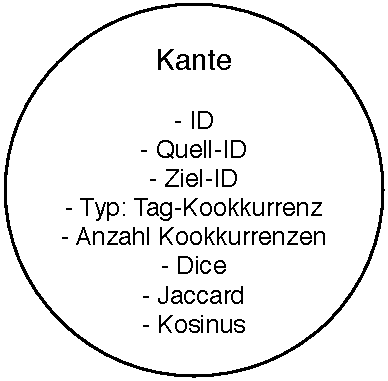
\includegraphics[width=0.3\textwidth]{tag_transform_edge}
\caption{Aufbau der aus den Tag-Daten erzeugten Kanten}
\label{fig:tag_transform_edge}
\end{figure}

\begin{lstlisting}[language=json, label={lst:tag_transform_edge}, caption={Tag-Kante als JSON-Dokument}]
{
    "_id" : ObjectId("51efd6f61177ff360605bd99"),
    "source" : ObjectId("51efc1af47cae77dfc00c3f8"),
    "target" : ObjectId("51efc1e047cae77dfc02087c"),
    "type" : "tag-co-occurence",
    "occurences" : 1,
    "dice" : 0.0001317089232795522,
    "jaccard" : 0.00006585879873551106,
    "cosine" : 0.008115343414514944
}
\end{lstlisting}

\subsection{Integration}

Da der aus den Tag-Daten generierte Kookkurrenzgraph die Ausgangsbasis für alle weiteren Operationen darstellt, muss im Sinne der Integration nichts getan werden. Die transformierten Daten müssen lediglich in die Zieldatenbank kopiert werden.

Durch die Schritte, die zur Link Discovery aus den Tag-Daten verwendet wurden, wurden insgesamt \num{314351} Knoten und \num{21834868} Kanten erzeugt, welche nun durch weitere Schritte angereichert werden sollen.

\section{Clicktracking}

Wie in \ref{problem:clicktracking} bereits einführend beschrieben, betreibt Spreadshirt ein Clicktracking-System, welches die Klicks der Benutzer auf Suchergebnisseiten aufzeichnet. Die von diesem System erzeugten Daten können für die Link Discovery von großer Bedeutung sein, da sie eine andere Perspektive auf die Begriffe im Graphen liefern. Die Tags liefern die Sicht der Partner, also der Personen, die Inhalte hochladen und verkaufen möchten. Die Klicks beschreiben die Sicht der Käufer, also der Personen, die nach Inhalten suchen. Durch die Auswertung der Clicktracking-Daten ergibt sich also die Möglichkeit, eine Form der Validierung der durch Partner vergebenen Metadaten zu erhalten. Die Annahme hierbei ist, dass Käufer nur auf Suchergebnisse klicken, die eine inhaltliche Relevanz zum eingegebenen Suchbegriff besitzen.

Wie bereits für die Tag-Daten, werden im Folgenden auch für das Clicktracking die Schritte Import, Bereinigung, Reduktion, Transformation und Integration näher erläutert. Der Ansatz zur Erzeugung der Verbindungen ist ebenfalls Kookkurrenzbasiert.

\subsection{Import}
\label{click_import}

Das Clicktracking-System erzeugt Dateien im JSON-Format, die zu jedem Klick auf einer Ergebnisseite die wesentlichen Informationen enthalten. Dabei ist pro Klick ein JSON-Dokument in der Datei abgespeichert. Ein Beispiel für ein solches Dokument ist in Listing \ref{lst:click_raw} dargestellt.

\begin{lstlisting}[language=json, label={lst:click_raw}, caption={Clicktracking - Rohdokument als JSON}]
{
    "date": "01.07.2013 00:09:31_633",
    "path": "/track/eu/205909/1E3B6E3E-B454-4496-C51A14A8FA25/2.10.4/list",
    "params": {
        "locale": "[de_DE]",
        "search-query": "[biene]",
        "cl": "[a18869874, p25446183, i49]"
    }
}
\end{lstlisting}

Ein Clicktracking-Dokument enthält dabei die Attribute \emph{Datum}, \emph{Pfad}, \emph{Gebietsschema}, \emph{Suchbegriff} und die Daten des eigentlichen Klicks, also den geklickten \emph{Artikel}, das geklickte \emph{Produkt} und den \emph{Index}, also die Position des geklickten Inhaltes auf der Suchergebnisseite. Die Unterscheidung zwischen Produkt und Artikel ist dabei im Domänenmodell von Spreadshirt begründet und für die Link Discovery nicht von Interesse. Es genügt, den geklickten Artikel im Weiteren näher zu betrachten.

Auffällig ist, dass die Möglichkeiten des JSON-Formates bei der Speicherung der Klickdaten nicht vollständig ausgenutzt wurden. So sind die Werte, die das geklickte Dokument beschreiben, als Zeichenkette abgelegt und zusätzlich die eindeutigen Bezeichner mit einem Buchstaben versehen, der ihren Typ angibt. Des weiteren enthalten  das Gebietsschema und der Suchbegriff zusätzliche eckige Klammern. Diese Defekte sollten im Bereinigungsschritt beseitigt werden, um ein nutzbareres Datenformat zu erhalten.

Da das Clicktracking-System zum Zeitpunkt des Imports erst 3 Monate Daten aufzeichnete, standen \num{2249942} solcher Klickdokumente zur Verfügung.

\subsection{Bereinigung}

Im Bereinigungsschritt müssen zunächst die genannten Defekte der Klickdaten beseitigt werden. Dazu gehört die Entfernung der eckigen Klammern in Suchbegriff und Gebietsschema und die Extraktion des eindeutigen Bezeichners des geklickten Artikels. Aus dem Gebietsschame ist nur die Sprache von Interesse. Außerdem wurden für den Suchbegriff die gleichen Bereinigungsoperationen wie für die Tag-Daten vorgenommen, also die Entfernung von überflüssigen Leerzeiche, Groß-/Kleinschreibung, nicht druckbarer Sonderzeichen und Satzzeichen.

Im Bereinigunsschritt werden so auch einfacher verarbeitbare Dokumente erzeugt, da die Möglichkeiten des JSON-Formates besser ausgenutzt werden. Listing \ref{lst:tag_cleanup} zeigt das Ergebnis der Bereinigung des in \ref{click_import} gezeigten Beispieldokumentes.

\begin{lstlisting}[language=json, label={lst:tag_cleanup}, caption={Bereinigtes Clicktracking-Dokument}]
{
    "_id": ObjectId("51e7b1e0417498f9c6868939"),
    "query" : "biene",
    "date" : "2013-07-01T00:09:31.633Z",
    "articleId" : 18869874,
    "index" : 57,
    "language" : "de"
}
\end{lstlisting}

\subsection{Reduktion}

Die Reduktion der Clicktracking-Daten besteht zum einen aus einer Duplikatentfernung, zum anderen aus der Einschränkung der Sprache.

Im Sinne der Kookkurrenz ist es nicht von Bedeutung, wenn Paare aus Suchbegriffen und geklickten Artikeln mehrfach auftauchen, da hierfür nur das gemeinsame Auftreten unterschiedlicher Suchbegriffe betrachtet wird. Somit besteht die Duplikatentfernung lediglich darin, aus mehrfach vorkommenden Artikel-/Klickpaaren genau eines auszuwählen.

Außerdem erfolgte, wie schon bei den Tag-Daten, eine Einschränkung auf Klicks, die als \emph{deutsch} gekennzeichnet sind.

Nach dem Reduktionsschritt verblieben zur Transformation noch \num{411341} Klicks.

\subsection{Transformation}

Im Transformationsschritt wird für die Clicktracking-Daten ein Kookkurrenzgraph berechnet. Die Kookkurrenz bestimmt sich hierbei daraus, welche Suchbegriffe zum Klick auf einen Artikel geführt haben. Wird ein Artikel zu mehreren Suchbegriffen geklickt, liegt die Vermutung nah, dass zwischen den Suchbegriffen ein irgendwie gearteter Zusammenhang besteht.

Ziel der Transformation ist somit die Erzeugung von Knoten und Kanten. Die Knoten besitzen dabei zusätzliche Eigenschaften, die die Eigenschaften des durch den Knoten repräsentierten Begriffes im Kontext des Clicktrackings widerspiegeln. Konkret sind dies die Artikel, die zu dem Begriff als Suchbegriff geklickt wurden. Listing \ref{lst:click_node} zeigt beispielhaft ein erzeugtes Knotendokument.

\begin{lstlisting}[language=json, label={lst:click_node}, caption={Knotendokument mit Clicktracking-Eigenschaften}]
{
    "_id": ObjectId("51e7f1e04146498f9c6868945"),
    "string": "biene",
    "language": "de",
    "clickProperties": [
        { "articleId": 4512 },
        { "articleId": 4794 },
        ...
    ]
}
\end{lstlisting}

Die Kanten besitzen die gleiche Form wie die Kookkurrenzkanten, die bei der Integration der Tag-Daten erzeugt wurden. Ein Beispiel für ein solches Kantendokument ist in Listing \ref{lst:click_edge} dargestellt.

\begin{lstlisting}[language=json, label={lst:click_edge}, caption={Clicktracking-Kookkurrenzkante}]
{
    "_id": ObjectId("51e91aff3b6a20bfd68c468a")
    "source" : ObjectId("51e91af93b6a20bfd68b0bed"),
    "target" : ObjectId("51e91aff3b6a20bfd68c463e"),
    "type": "tag-co-occurence",
    "occs" : 1,
    "dice" : 0.003883495145631068,
    "jaccard" : 0.0019455252918287938,
    "cosine" : 0.04410810913912309
}
\end{lstlisting}

Die Durchführung des Transformationsschrittes erfolgte ebenfalls mittels MapReduce (siehe \ref{mapreduce_cooccurence}). Dadurch wurden \num{92727} Knoten und \num{310860} Kanten erzeugt.

\subsection{Integration}

Die Integration der erzeugten Daten stellt eine Vereinigung des vorhandenen Zielgraphen mit dem im Transformationsschritt erzeugten Kookkurrenzgraphen dar.

Dabei wird die Knotenmenge derart vereinigt, dass die Knotenmenge des Zielgraphen die Eigenschaft behält, dass Paare aus Sprache und Zeichenkette eindeutig sind. Somit werden bei bereits vorhandenen Knoten die zusätzlichen Informationen bezüglich das Clicktrackings als Attribute hinzugefügt. Existiert eine Kombination aus Sprache und Zeichenkette noch nicht im Zielgraph, so wird der entsprechende Knoten kopiert.

Da die erzeugten Kanten einen noch nicht im Graoh vorhandenen Typ besitzen, müssen keine Kanten zusammengeführt werden. Jedoch müssen die Ziel- und Quellquoten entsprechend angepasst werden, wenn bei der Integration der Knoten eine Zusammenführung statt gefunden hat.

Durch dieses Vorgehen konnten der Knotenmenge \emph{78237} Knoten, und somit auch neue Begriffe hinzugefügt werden. Die Kantenmenge wurde, wie bereits erläutert, um \emph{310860} Kanten erweitert.

\section{Google Translate}

Google bietet im Rahmen seines \emph{Translate}-Services \cite{gt2013} eine kostenpfichtige API für Spracherkennung an. Diese ermöglicht es, die Sprache beliebiger Zeichenketten automatisch erkennen zu lassen. Google stellt hierzu eine REST-API zur Verfügung.

Diese Schnittstelle liefert Ergebnisse der Form \((l, c)\), wobei \(l\) die für die Zeichenkette erkannte Sprache und \(c\) einen Konfidenzwert für die Spracherkennung repräsentiert. Der Konfidenzwert liegt dabei im Intervall zwischen \num{0} und \num{1} und stellt die Verlässlichkeit der Spracherkennung dar.

Die Integration der Spracherkennungs-Daten in den Graphen gestaltet sich einfach. Dazu werden die durch die bereits vorhandenen Knoten repräsentierten Zeichenketten extrahiert und als Eingabedaten für die Spracherkennungs-API verwendet. Die Ergebnisse werden abgespeichert, um weitere kostenpflichtige Abfragen zu vermeiden.

Eine Bereinigung der Ergebnisse ist nicht erforderlich. Somit müssen die Ergebnisse lediglich in den Ausgangsgraphen integriert werden. Die Spracherkennung an sich bringt keine Ähnlichkeitsbeziehungen mit sich, sondern verbessert gegebenenfalls nur die Knotenauswahl für spätere Operationen.

In der Konsequenz genügt es also, die für die Abfrage verwendeten Knoten mit den Ergbenissen der Spracherkennung zu annotieren. Somit kann dann bei späteren Analysen anhand des Konfidenzwertes abgewogen werden, ob die erkannte Sprache oder die eventuell schon am Knoten vorhandene Sprache verwendet werden soll.

\section{Zerlegung von Wortgruppen}

Die Zerlegung von Tags, die aus mehr als einem Wort bestehen, stellt zwar keine Integration anderer Datenquellen dar, kann aber trotzdem zum Auffinden neuer Verknüpfungen nützlich sein.

Zum Zeitpunkt des Importes befanden sich \num{147364} Tags in der Datenbank, die aus mehreren Wörtern bestehen. Dies entspricht \num{47} Prozenzt aller bereinigten deutschen Tags. Dieser Umstand legt die Vermutung nahe, dass in diesen zusammengesetzten Tags auch Wörter enthalten sind, die nicht als Einzelwörter existieren.

Werden diese Tags in ihre Einzelwörter zerlegt, entstehen einerseits unter Umständen neue Knoten, andererseits können in diesem Schritt Kanten vom Typ \emph{Zerlegung} beziehungsweise \emph{Zusammensetzung} eingefügt werden. Somit sind nach dem Zerlegungsschritt weitere Informationen über den Kontext, in dem Wörter verwendet werden, verfügbar. Abbildung \ref{fig:decomposition} zeigt beispielhaft das Ergebnis einer solchen Zerlegung.

Durch die Anwendung des Zerlegungsschrittes auf die vorhandenen Tag-Daten wurden insgesamt \num{38349} Knoten und \num{1238900} Kanten erzeugt, die für spätere Analyseschritte genutzt werden können.

\begin{figure}
\centering
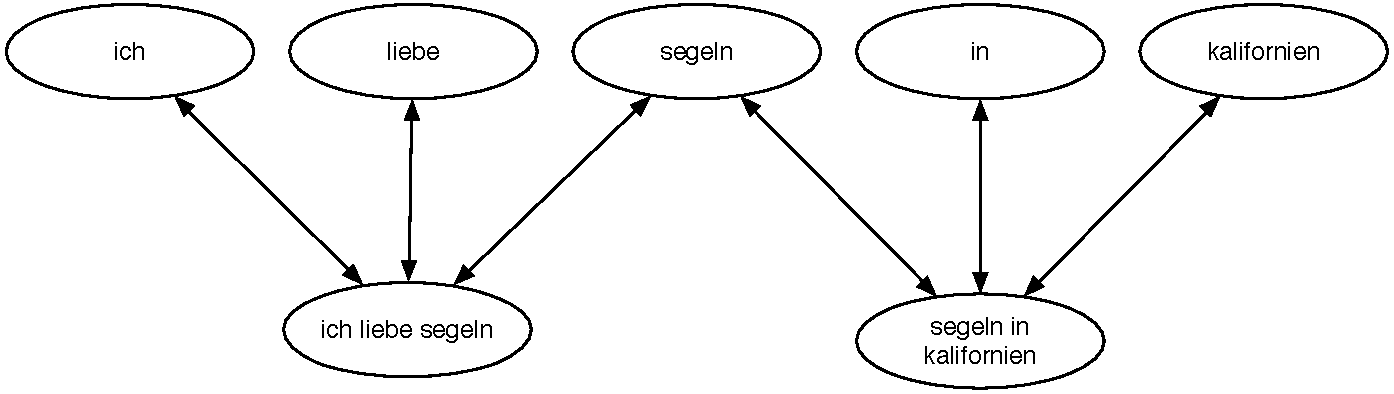
\includegraphics[width=\textwidth]{decomposition}
\caption{Beispielhafter Graphausschnitt nach der Zerlegung}
\label{fig:decomposition}
\end{figure}

\section{Wortschatz der Universität Leipzig}

Die Universität Leipzig betreibt ein Wortschatz-Projekt \cite{ws2013}. Im Rahmen dieses Projektes wird durch die Analyse von großen Textmengen eine Datenbank deutscher Wörter, deren Bedeutungen, grammatikalische Eigenschaften, Häufigkeiten und Kookkurrenzen in Texten und Beziehungen zu anderen Wörtern aufgebaut. Somit stellt dieses Projekt eine sehr gute Möglichkeit dar, weitere Beziehungen zwischen den schon im Graph vorhandenen Knoten herzustellen. Neben den Daten, die im Spreadshirt-Kontext entstehen, können somit auch allgemeine linguistische Daten hinzugefügt und für spätere Analysen genutzt werden.

Neben dem Webportal stellt dieses Projekt eine SOAP-API bereit, über die die Daten des Wortschatz programmatisch abgefragt werden können. Diese API wurde mittels einer Ruby-Bibliothek \cite{wlapi2013} im Rahmen dieser Arbeit für einen weiteren Integrationsschritt zur Link Discovery genutzt.

Für jedes Wort als Eingabeparameter stellt die Wortschatz-API die folgenden Informationen bereit:

\begin{itemize}
    \item Grundform des Wortes
    \item Wortformen
    \item Kookkurrenzen in den analysierten Texten
    \item Kategorien, in die das Wort eingeordnet werden kann
    \item Synonyme
    \item Thesaurus-Beziehungen
    \item Häufigkeit des Auftretens
    \item Sätze, die das Wort enthalten
\end{itemize}

Für die Link Discovery wurden die die Informationen \emph{Grundform}, \emph{Wortformen}, \emph{Kategorien}, \emph{Synonyme} und \emph{Thesaurus-Beziehungen} genutzt.

Wie bereits für die anderen Datenquellen, werden im Folgenden auch für den Wortschatz die Schritte des Imports, der Bereinigung, der Reduktion, der Transformation und der Integration beschrieben.Wie bereits für die anderen Datenquellen, werden im Folgenden auch für den Wortschatz die Schritte des Imports, der Bereinigung, der Reduktion, der Transformation und der Integration beschrieben.

\subsection{Import}

Da für die Anfrage an die Wortschatz-API nur Einzelwörter und keine Wortgruppen genutzt werden können, muss eine Auswahl der anzufragenden Daten getroffen werden. Im Rahmen dieser Arbeit wurden alle Einzelwörter, die zum Zeitpunkt des Importes der Wortschatz-API zur Verfügung standen, ausgewählt. Dabei handelt es sich um \num{197614} einzelne Wörter. Da die Daten in der Datenbank zu diesem Zeitpunkt keine Groß- und Kleinschreibung enthielten, die Wortschatz-API diese jedoch berücksichtigt, wurde jedes Wort jeweils groß und klein geschrieben angefragt. Somit wurde die doppelte Menge an Datensätzen, \num{395228} Dokumente, erzeugt.

Die Ergebnisse wurden mittels eines Ruby-Skriptes in MongoDB importiert. Dabei wurde je angefragtem Wort ein Dokument erzeugt, dass die Wortschatz-Informationen enthält. Eines dieser Dokumente ist beispielhaft in Listing \ref{lst:wortschatz_import} dargestellt. Das Feld \emph{baseform} enthält dabei die Grundform des Wortes mit der Wortart und \emph{domain} die Kategorien des Wortes.

\begin{lstlisting}[language=json, label={lst:wortschatz_import}, caption={Wortschatz-Dokument nach dem Import}]
{
    "_id" : ObjectId("51f7aa06eba16044e900015a"),
    "string" : "Kopf",
    "baseform" : [ 
        "Kopf", 
        "N"
    ],
    "domain" : [ 
        "Medizin", 
        "Anatomie", 
        "Literarische/Motive/Stoffe/Gestalten", 
        "Körperteile"
    ],
    "synonyms" : [  
        "Chef", 
        "Figur", 
        "Gestalt", 
        "Haupt", 
        "Jemand", 
        "Individuum", 
        "Figur"
    ],
    "thesaurus" : [ 
        "Titel", 
        "Hand", 
        "Kopf", 
        "Mensch", 
        "Gesicht", 
        "Spitze", 
        "Arm", 
        "Gestalt"
    ],
    "wordforms" : [ 
        "Kopf", 
        "Köpfe", 
        "Köpfen", 
        "Kopfes", 
        "Kopfs"
    ]
}
\end{lstlisting}

Hierbei ist zu beachten, dass nicht alle Attribute bei allen Wörtern vorhanden sind. Dies hängt davon ab, ob der Wortschatz die Informationen zur Verfügung stellen kann. Somit ist es auch möglich, dass Dokumente erzeugt werden, die keine zusätzlichen Informationen enthalten.

\subsection{Bereinigung}

Zur Bereinigung der importierten Wortschatz-Daten muss in einem ersten Schritt die Groß- und Kleinschreibung entfernt werden, da diese an erster Stelle nur für die Anfragen an die API wieder in den Datenbestand eingeführt wurde.

Weiterhin werden die Kategorien ``Vorname'' und ``Nachname'' entfernt, da diese an über \num{25000} Wörter vergeben sind und somit für die Verwendung zur Link Discovery ungeeignet sind und zu viele irrelevante Kanten erzeugen würden.

Ein letzer Bereinigungsschritt besteht in der Veränderungen des Formates der Grundform des Wortes. Die Wortschatz-API liefert lediglich ein Array, in dem das erste Element die Grundform und das zweite Element die Wortart ist. Zur Bereinigung wird diese Eigenschaft in ein geeignetes JSON-Format überführt, welches in Listing \ref{lst:word_baseform} dargestellt ist.

\begin{lstlisting}[language=json, label={lst:word_baseform}, caption={Grundform eines Wortes}]
{
    _id: ...,
    string: "Kopfs",
    baseform: {
        word: "Kopf",
        type: "N"
    }
}
\end{lstlisting}
